\documentclass{comjnl}

\usepackage{amsmath}
\usepackage{hyperref}
\newcommand*\chem[1]{\ensuremath{\mathrm{#1}}}

%% These two lines are needed to get the correct paper size
%% in TeX Live 2016
\let\pdfpageheight\paperheight
\let\pdfpagewidth\paperwidth

%\copyrightyear{2009} \vol{00} \issue{0} \DOI{000}

\begin{document}

\title[Granular superconductivity of Rutherford cable and cuprate/manganite multilayer]{How superconductivity in Rutherford MgB2 Cables and cuprate/manganite multilayer is affected by external factors}
\author{Even M. Nordhagen}
\affiliation{Computational physics group, Department of Physics, University of Oslo, Oslo, Norway} \email{evenmn@fys.uio.no}

\shortauthors{E. M. Nordhagen}
 
\received{00 November 2017}
\revised{00 Month 2017}


%\category{C.2}{Computer Communication Networks}{Computer Networks}
%\category{C.4}{Performance of Systems}{Analytical Models}
%\category{G.3}{Stochastic Processes}{Queueing Systems}
%\terms{Internet Technologies, E-Commerce}
\keywords{Granular superconductivity; Rutherford cable; Cuprate; Manganite; Transport measurements; Magneto Optical Imaging}


\begin{abstract}
We investigate the superconductive properties of 12 twisted Rutherford \chem{MgB_2} cables and 10 layers of \chem{Pr_{0.5}La_{0.2}Ca_{0.3}MnO_3/YBa_2Cu_3O_7} (PLCMO/YBCO) using magneto-optical imaging and transport measurements, with the latter as the main focus. The transport measurements were done carefully, where we studied how the resistance and current through the sample was affected by the temperature. Liquid helium was used to cool down the sample to lower temperatures (minimum 3.7 Kelvin), and for a bit higher temperatures we used liquid nitrogen (minimum 77 Kelvin). For comparison a single-layer PLCMO/YBCO was investigated by transport measurements. Furthermore magneto-optical imaging was inducted for all the samples, but unfortunately only the Rutherford tape gave good results.
\end{abstract}

\maketitle


\section{Introduction}
In 1879 Thomas Edison produced the first reliable, long-lasting electric bulb, and immediately .. Every year since the network of .. has been expanded, annually of a length ... Those conductors have resistance, which cause energy loss. 

At the same time we are burning huge amounts of oil to get energy, essentially for electricity or transport usage. Exactly how much oil is remaining on Earth is unknown, and how much we can make use of depends on the future technology. Anyway what is sure is that it will not last forever, and we need to find new, probably renewable, energy sources. What if we could find a renewable energy carrier which was so cold that it could cause superconductivity at the same time? We do not need to search further, the solution is liquid hydrogen! When hydrogen reacts with oxygen, we get water, which is 100\% renewable, at the same time as liquid hydrogen has a temperature of 20K. 

We need a material which is superconducting above 20K, which can be made in large scales, and \chem{MgB_2} seems to be promising. Among others we have investigated a Rutherford cable (which has a core of \chem{MgB_2}).

\section{Theory}\label{Sec:Theory}
Superconductive materials have two main properties: They are resistance-free conductors under a critical temperature $T_c$ and magnetic field cannot penetrate the material under the same temperature $T_c$. The methods we gonna make use of both these main properties. Perhaps the easiest way to find the resistance of a sample is to connect the sample to a power supply and measure the voltage difference, $U$, between two points. The resistance can then be calculated by Ohm's law $U=RI$, given the current $I$. This is known as a four-point measurement or four-terminal sensing, and is widely used in transport measurements. No voltage drop corresponds to zero resistance. In figure (\ref{fig:onnes_1911}) one can find a sketch of a four-point measurement. 

In some cases it is appropriate to use more advanced techniques, for instance when the sample structure is not uniform in every direction. Then we might want to measure the resistance in various directions, but without disturbing the samples with more contacts than necessary. By placing the contacts in each corner, we can reuse the contacts when "turning" the sample, known as the .. , illustrated in figure (..). 

\begin{figure}[h]
\centering
\includegraphics[width=50mm]{onnes_1911.jpg}
\caption{RT-graph drawn by Kamerlingh Onnes in 1911. Image downloaded from wikipedia \url{https://commons.wikimedia.org/wiki/File:Superconductivity_1911.gif} \label{fig:onnes_1911}}
\end{figure}

\section{Methods}\label{Sec:Methods}
We will examine the samples using mainly two methods: Transport measurements and magneto optical imaging

\subsection{Transport Measurements (TM)}
Transport measurements is the simplest of the two methods and will be our main method. As the name indicates, TM is all about set current to the sample and measure voltage drop. A standard TM is done by connecting current cables on the outermost connecting points and two voltage cables in between as illustrated in figure (...). The connections are made by Indium (In) since it is a good conductor and easy to distribute, i.e ...

\subsection{Magneto-Optical Imaging (MOI)}
Our eyes are not able to see magnetism, but with a MOI apparatus we can take pictures of a superconductor and decide if a sample is superconducting using the elementary magnetic property discussed in section \ref{Sec:Theory}. The method is quite in-complicated where light is reflected by a Faraday crystal on top of the sample. If the Faraday crystal is affected by a magnetic field, it will polarize the light, and it will later be separated out by a polarization filter, as shown in figure (\ref{fig:MOI}). The idea is that all the light will go through the filter as long as the sample is not superconducting. Alternatively if the sample is superconducting, we will get no light passing in the superconducting area. Not only can MOI detect superconductivity, but we can also see exactly where the material is superconducting, which is convenient for non-homogeneous materials. 
\begin{figure}[h]
\centering
\includegraphics[width=50mm]{MOI.jpg}
\caption{General setup of MOI. Image is taken from wikipedia \url{http://www.mn.uio.no/fysikk/english/research/groups/amks/superconductivity/mo/} \label{fig:MOI}}
\end{figure}
We inducted MOI on 

\section{Experiments} \label{Sec:Experiments}
The experiments were implemented in the same way for both the samples, so unless there are reasonable differences, I will present the general approach

\subsection{TM}
-Place sample on "finger"
-The currents were attached by indium to get optimal conductivity between sample and currents
-Attach sample using several layers of tape (works also as protection)
-Strap thread around the tape to make sure it will not loosen
-Cut a finger of a vinyl glow, and strap it around the tape. This works as an isolation mechanism, in the same time as it keeps the fluid outside. With no isolation the temperature will simply decrease too fast.
-Dip the sample into the liquid and measure the temperature and drop in voltage.

\subsection{MOI}
Placed sample on sampleholder
Place Faraday crystal on sample
Mount stabilizators
Make vacuum (below 1e-4 mPa)
Cool down to working temp
Can use heater 
Change current and polarization
Take pictures


\section{Results}  \label{Sec:Results}
\subsection{Rutherford cable}


\subsection{YBCMO multilayer}
\begin{figure}[h]
\centering
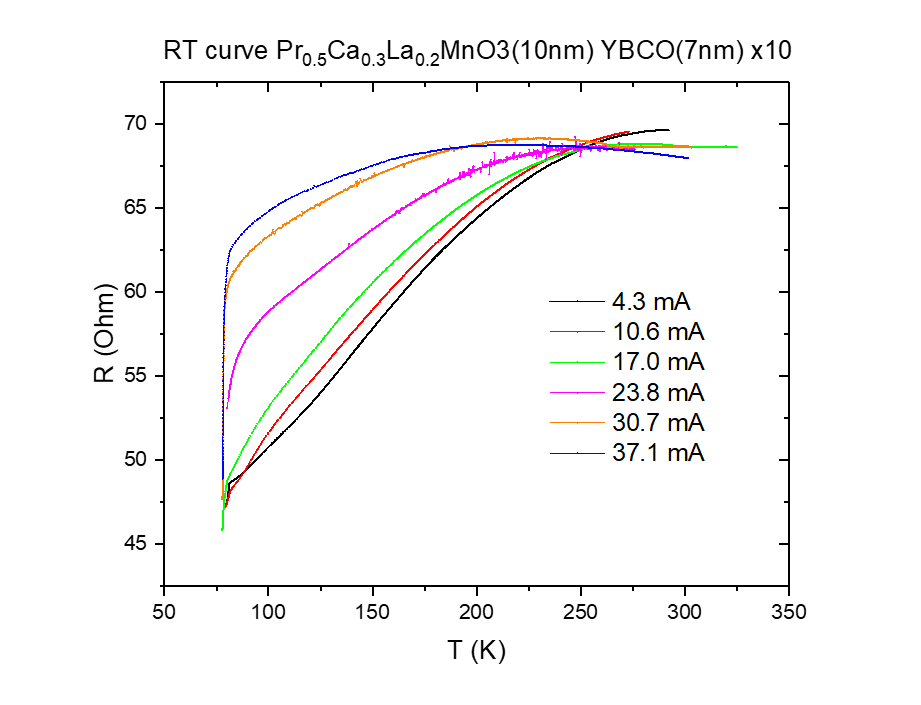
\includegraphics[width=100mm]{Bilde1.png}
\caption{INSERT CAPTION \label{fig:MOI}}
\end{figure}

\begin{figure}[h]
\centering
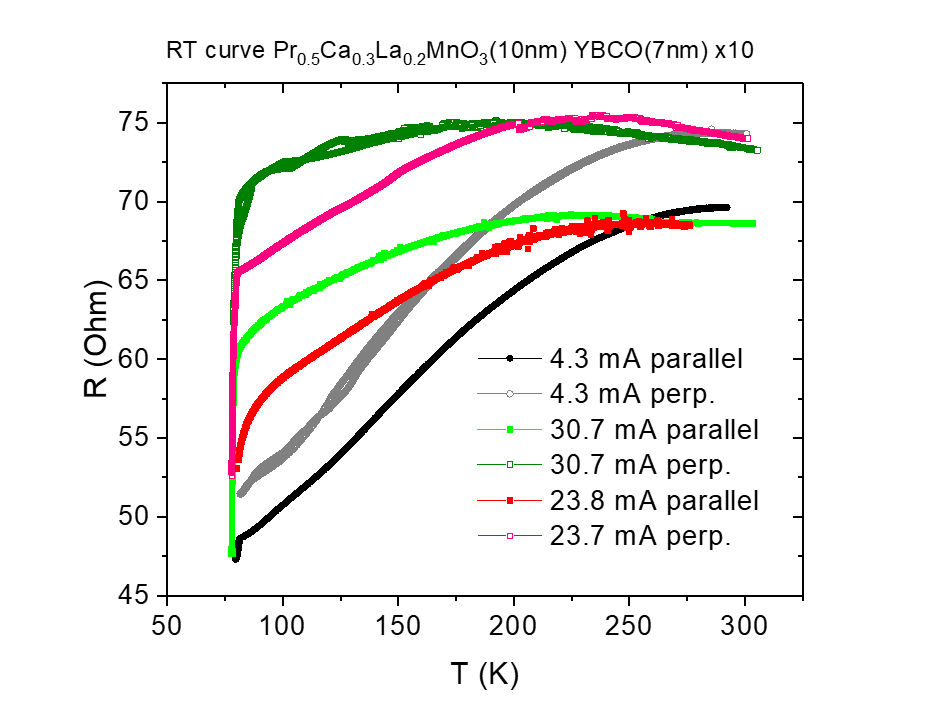
\includegraphics[width=100mm]{Bilde2.png}
\caption{INSERT CAPTION \label{fig:MOI}}
\end{figure}

\begin{figure}[h]
\centering
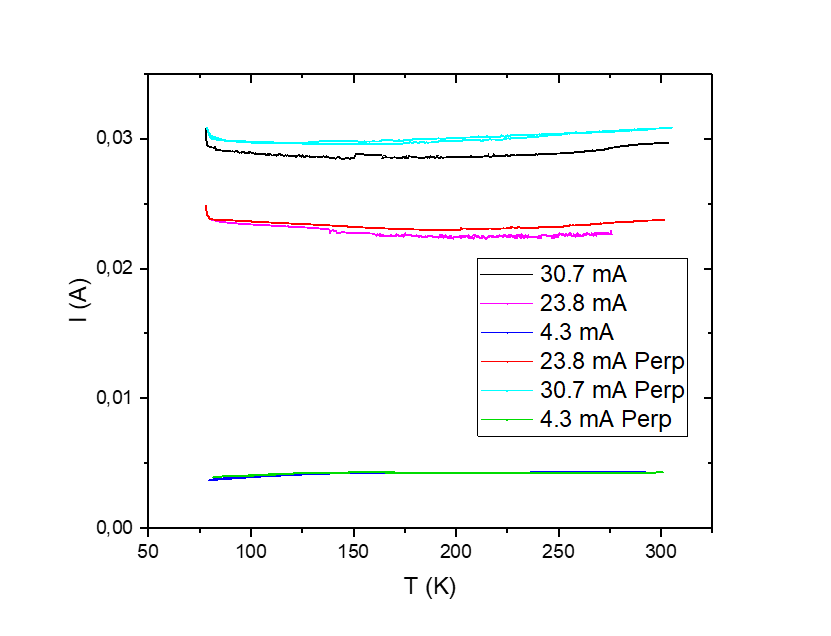
\includegraphics[width=100mm]{Bilde3.png}
\caption{INSERT CAPTION \label{fig:MOI}}
\end{figure}

\begin{figure}[h]
\centering
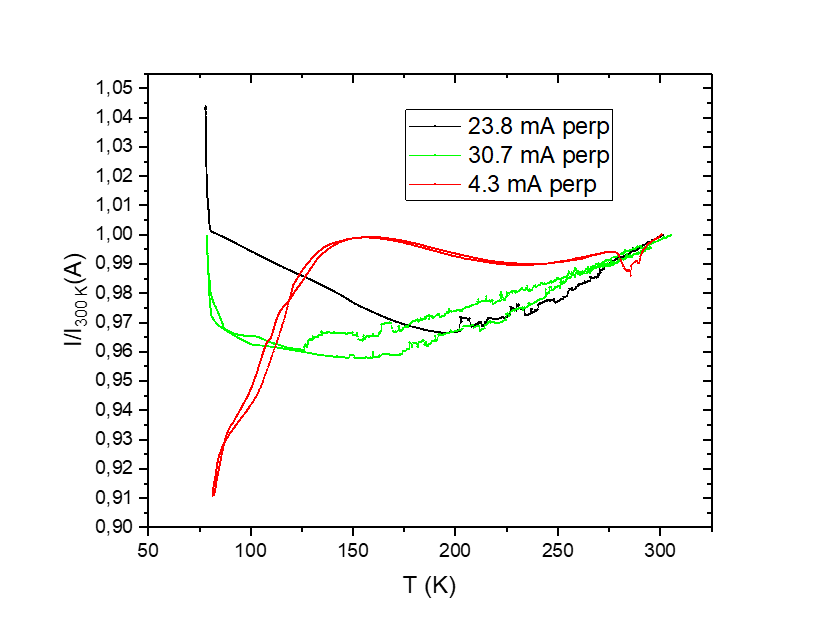
\includegraphics[width=100mm]{Bilde4.png}
\caption{INSERT CAPTION \label{fig:MOI}}
\end{figure}

\subsection{YBCMO single-layer}
For comparing

\section{Conclusion} \label{Sec:Conclusion}

\ack{This research was undertaken as part of the ALADDIN
(Autonomous Learning Agents for Decentralised Data and Information
Networks) project and is jointly funded by a BAE Systems and EPSRC
(Engineering and Physical Research Council) strategic partnership
(EP/C548051/1).}


\nocite{*}

\bibliographystyle{compj}
\bibliography{ModellingBidders}


\end{document}